\newpage
\section{Results}
\begin{figure*}[h]
    \begin{minipage}[t]{0.32\textwidth}
        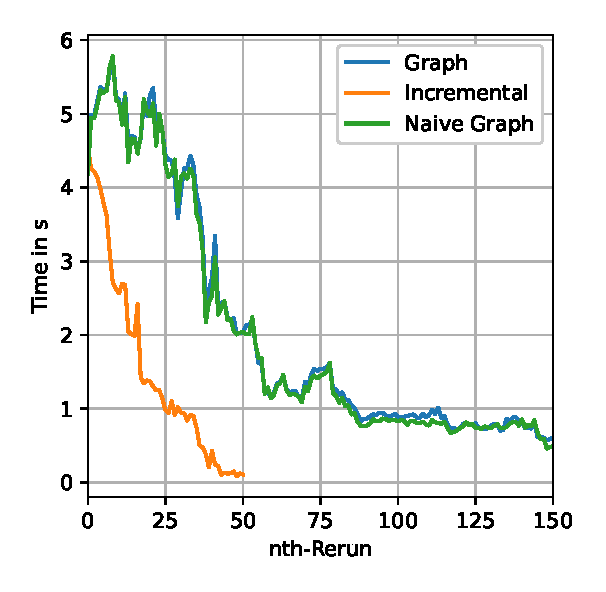
\includegraphics[width=1\textwidth]{benchmarking/sparse_rerun_cropped.eps}
    \end{minipage}
    \begin{minipage}[t]{0.34\textwidth}
        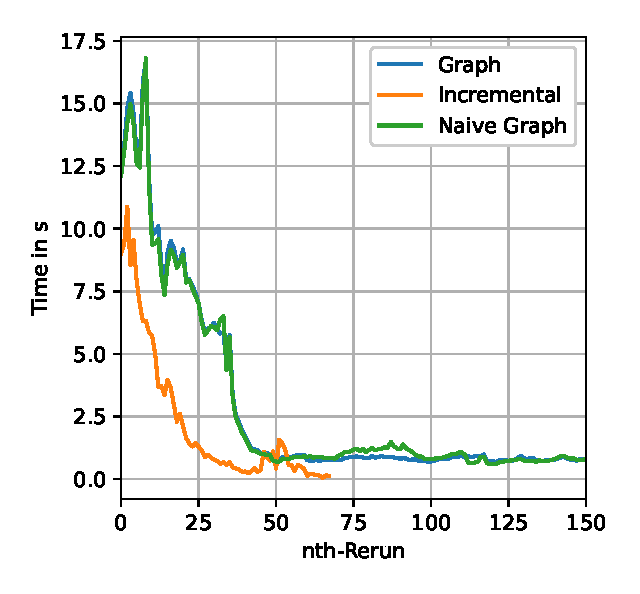
\includegraphics[width=1\textwidth]{benchmarking/medium_rerun_cropped.eps}
    \end{minipage}
    \begin{minipage}[t]{0.32\textwidth}
        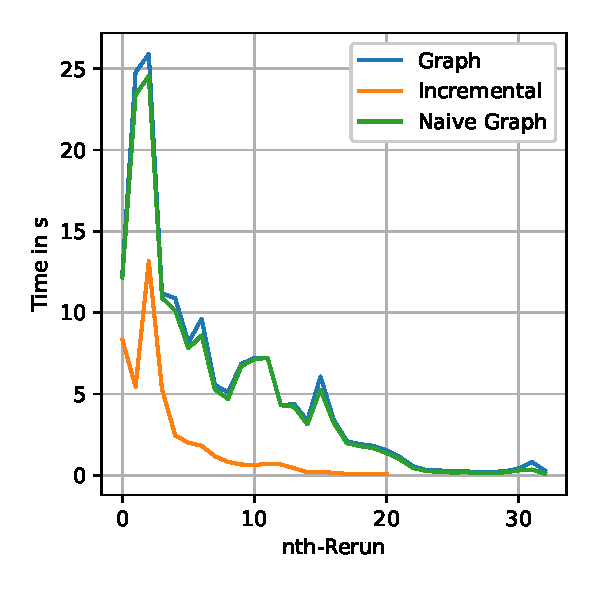
\includegraphics[width=1\textwidth]{benchmarking/dense_rerun_cropped.eps}
    \end{minipage}
    \caption{Time cost over rerun (from left to right sparse, medium, dense)}
    \label{fig:cropped}
\end{figure*}

As visible in Figure \ref{fig:cropped} our hypothesis, that the graph approach might have problems with an escalating window, did not hold true. The figures show, the timen take for all reruns, averaged over all sparse, medium and dense instances.

\begin{figure*}[h]
	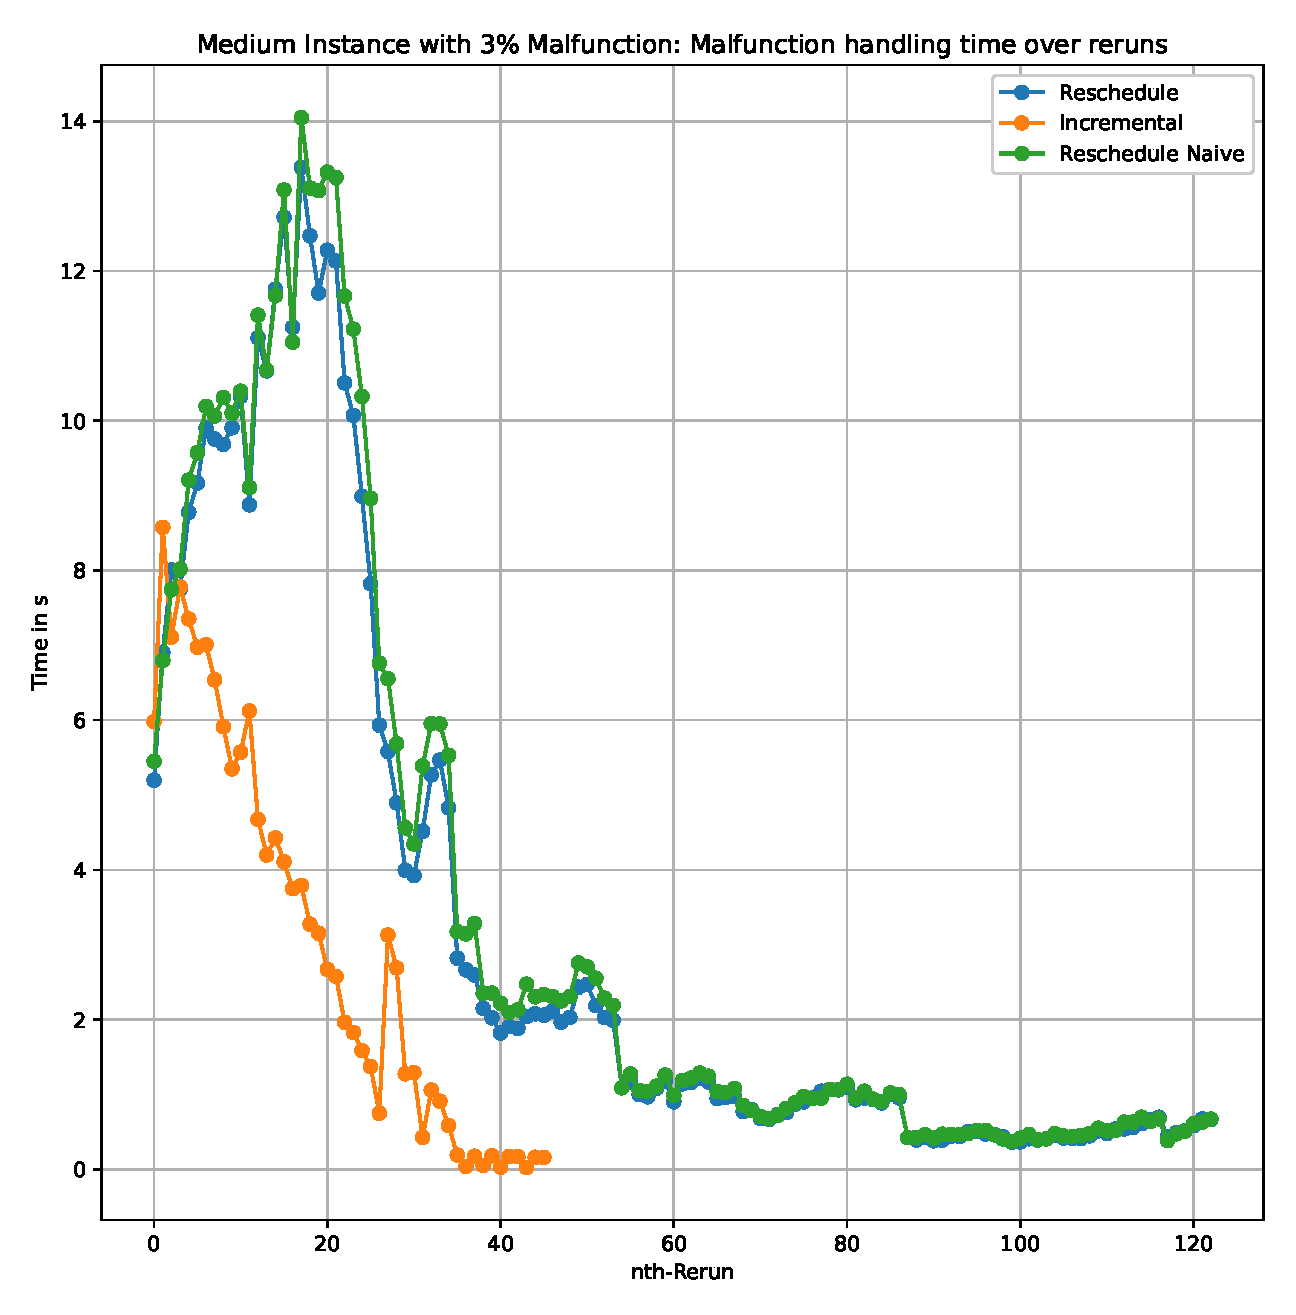
\includegraphics[width=1\textwidth]{benchmarking/medium_3_4_rerun_full.eps}
	\caption{A singular medium Instance with 3\% Malfunction}
	\label{fig:medium_instance}
\end{figure*}


As Figure \ref{fig:medium_instance} illustrates, the first reruns have a growing time consumption (in the example up to the 20th rerun), but after some trains have reached their goals, the rerun time decreases as does the window, due to fewer malfunctions. It is still not the most efficient solution, as the incremental approach illustrates, but the scaling is not as bad as expected.

The hypothesis, that the malfunction handling of the Graph approach works worse for malfunction dense environments, did not hold. The hypothesis was, that the extension of the horizon for the Graph performs worse with more malfunctions. Taking incremental as a comparison, one can see, that the graph approach performs better in the dense setting, thus refuting our assumption. We did not take into account, that more malfunctions also tend to approach the worst case, and thus improve the performance of the approach relatively.

Our assumption that the naive approach would perform worse than the graph approach did not hold. It seems, that computing the graph is similarly efficient as reading the graph from input, with most instances performing slightly better, if the graph is recomputed (naive). There was no significant difference even on sparse instances. As we can see in the long tail the grounding of the graph is under a second.

But the assumption, of the incremental outperforming the other approaches did hold. It shows shorter runtimes over all instances, also requiring less reruns, as it's solutions always use the optimal horizon. The window is shrinking on every rerun and only extended if required. One can spot the reruns, where more timesteps were necessary, by looking at the peaks in Figure \ref{fig:medium_instance}.

We can see a nice logarithmic curve, due to the nature of NP problems, as each choice prunes the search space.